\documentclass[hidelinks,12pt]{article}
\usepackage[left=0.25cm,top=1cm,right=0.25cm,bottom=1cm]{geometry}
%\usepackage[landscape]{geometry}
\textwidth = 20cm
\hoffset = -1cm
\usepackage[utf8]{inputenc}
\usepackage[spanish,es-tabla]{babel}
\usepackage[autostyle,spanish=mexican]{csquotes}
\usepackage[tbtags]{amsmath}
\usepackage{nccmath}
\usepackage{amsthm}
\usepackage{amssymb}
\usepackage{mathrsfs}
\usepackage{graphicx}
\usepackage{subfig}
\usepackage{standalone}
\usepackage[outdir=./Imagenes/]{epstopdf}
\usepackage{siunitx}
\usepackage{physics}
\usepackage{color}
\usepackage{float}
\usepackage{hyperref}
\usepackage{multicol}
%\usepackage{milista}
\usepackage{anyfontsize}
\usepackage{anysize}
%\usepackage{enumerate}
\usepackage[shortlabels]{enumitem}
\usepackage{capt-of}
\usepackage{bm}
\usepackage{relsize}
\usepackage{placeins}
\usepackage{empheq}
\usepackage{cancel}
\usepackage{wrapfig}
\usepackage[flushleft]{threeparttable}
\usepackage{makecell}
\usepackage{fancyhdr}
\usepackage{tikz}
\usepackage{bigints}
\usepackage{scalerel}
\usepackage{pgfplots}
\usepackage{pdflscape}
\pgfplotsset{compat=1.16}
\spanishdecimal{.}
\renewcommand{\baselinestretch}{1.5} 
\renewcommand\labelenumii{\theenumi.{\arabic{enumii}})}
\newcommand{\ptilde}[1]{\ensuremath{{#1}^{\prime}}}
\newcommand{\stilde}[1]{\ensuremath{{#1}^{\prime \prime}}}
\newcommand{\ttilde}[1]{\ensuremath{{#1}^{\prime \prime \prime}}}
\newcommand{\ntilde}[2]{\ensuremath{{#1}^{(#2)}}}

\newtheorem{defi}{{\it Definición}}[section]
\newtheorem{teo}{{\it Teorema}}[section]
\newtheorem{ejemplo}{{\it Ejemplo}}[section]
\newtheorem{propiedad}{{\it Propiedad}}[section]
\newtheorem{lema}{{\it Lema}}[section]
\newtheorem{cor}{Corolario}
\newtheorem{ejer}{Ejercicio}[section]

\newlist{milista}{enumerate}{2}
\setlist[milista,1]{label=\arabic*)}
\setlist[milista,2]{label=\arabic{milistai}.\arabic*)}
\newlength{\depthofsumsign}
\setlength{\depthofsumsign}{\depthof{$\sum$}}
\newcommand{\nsum}[1][1.4]{% only for \displaystyle
    \mathop{%
        \raisebox
            {-#1\depthofsumsign+1\depthofsumsign}
            {\scalebox
                {#1}
                {$\displaystyle\sum$}%
            }
    }
}
\def\scaleint#1{\vcenter{\hbox{\scaleto[3ex]{\displaystyle\int}{#1}}}}
\def\bs{\mkern-12mu}


\usepackage{apacite}
\title{3 - Construcción de un sistema coordenado especial \\[0.3em]  \large{Matemáticas Avanzadas de la Física}\vspace{-3ex}}
\author{M. en C. Gustavo Contreras Mayén}
\date{ }
\begin{document}
\vspace{-4cm}
\maketitle
\fontsize{14}{14}\selectfont
\tableofcontents
\newpage
\section{Construcción de sistemas coordenados.}
\subsection{Introducción.}
Una pregunta importante que planteamos en este momento es: ¿para qué estamos revisando los sistemas coordenados curvílineos?
\par
Como respuesta presentamos la siguiente: Ante un problema de la física, debemos de seleccionar el sistema coordenado de modo que se adapte al problema, \emph{para aprovechar cualquier oportunidad o simetría presente en el mismo}.
\par
De tal manera que resultará más fácil la solución que cuando se obliga a adaptar una solución en un sistema cartesiano.
\par
Cuando se menciona que \enquote{es más fácil la solución}, significa que se tendrá una ecuación diferencial parcial (EDP) que puede separarse en ecuaciones diferenciales ordinarias (EDO), frecuentemente en la \enquote{forma estándar} en el nuevo sistema coordenado.
\par
La \emph{técnica de separación de variables}, se verá en el Tema 2 del curso.
\subsection{Sistemas coordenados especiales.}
Conocemos al menos tres sistemas coordenados con los que hemos trabajado en distintas áreas de nuestra carrera: cartesiano, cilíndrico (en 3D, polar en 2D) y esférico.
\par
De manera conveniente enlistamos catorce sistemas coordenados, que en algún momento nos podremos encontrar.
\par
Como punto importante debemos de señalar que no es intención de curso que se haga una revisión completa, detallada para cada uno de los sistemas.
\par
Más bien, veremos una metodología con la cual abordaremos el estudio de un sistema coordenado, y entonces tendremos la manera de estudiar otros de acuerdo a las necesidades que se nos presenten.
\par
De manera conveniente se presenta una lista con catorce sistemas, clasificando los mismos de acuerdo con el hecho de que tengan o no:
\begin{enumerate}
\item Un eje de traslación (perpendicular a la familia de superficies de plano paralelo)
\item Un eje de simetría rotacional.
\end{enumerate}
{\fontsize{8}{8}\selectfont
\renewcommand{\arraystretch}{1.2}
\begin{table}[H]
\centering
\begin{tabular}{p{4cm} p{5.5cm} p{4cm}}
Eje de traslación & Eje de rotación & Ninguno \\ \hline
Cartesiano ($3$ ejes) & & Confocal elipsoidal \\
Circular cilíndrico & Circular cilíndrico & \\
& Polar esferoidal ($3$ ejes) & \\
Elíptico cilíndrico & Esferoidal prolato o alargado & \\
& Esferoidal oblato & \\
Parabólico cilíndrico & Parabólico & \\
Bipolar & Toroidal & \\
& Biesférico & \\[0.5em]
& & Cónico \\
& & Confocal paraboidal \\
\end{tabular}
\end{table}
}
El espaciamiento en la tabla indica las relaciones entre los diversos sistemas coordenados.
\par
Si se considera el caso en dos dimensiones ($z = 0$) de un sistema con un eje de traslación (columna izquierda) y se le hace girar alrededor de un eje de simentría de reflexión, se genera el sistema coordenado correspondiente indicado en la columna central hacia la derecha.
\par
Por ejemplo: la rotación del plano $z = 0$ del sistema cilíndrico elíptico alrededor del eje principal genera el sistema esferoidal alargado; la rotación alrededor del eje menor resulta en el sistema esferoidal oblato. También se consideran tres sistemas que no tienen eje de traslación o eje de rotación.
\par
En este grupo asimétrico, el sistema elipsoidal confocal se utiliza algunas veces como el sistema más general y del que casi todos los demás sistemas se obtienen del mismo.
\section{Desarrollo de un sistema coordenado.}
\subsection{Coord. cilíndricas elípticas \texorpdfstring{$(u, v, z)$}{(u, v, z)}}
A continuación veremos la manera de abordar un sistema coordenado especial, para determinar los las superficies constantes, los factores de escala, los operadores diferenciales, necesarios para resolver un problema con esta geometría en particular.
\subsection{Reglas de transformación.}
Para el sistema cilíndrico elíptico, se tienen las siguientes reglas de transformación:
\begin{align}
\begin{aligned}
x &= a \, \cosh u \, \cos v \\
y &= a \, \sinh u \, \sin v \\
z &= z
\end{aligned}
\label{eq:ecuacion_02_73_esp}
\end{align}
\subsection{Superficies coordenadas}
Para identificar las superficies constantes, elevamos al cuadrado cada lado
\begin{align}
x^{2} &= a^{2} \, \cosh^{2} u \, \cos^{2} v \label{eq:ecuacion_02_74_esp} \\
y^{2} &= a^{2} \, \sinh^{2} u \, \sin^{2} v \label{eq:ecuacion_02_75_esp}
\end{align}
Dividimos la primera expresión entre $\cos^{2} v$ y la segunda entre $\sin^{2} v$, recordando que $cos^{2} + \sin^{2} = 1$, así llegamos a
\begin{align}
\dfrac{x^{2}}{a^{2} \, \cosh^{2}} + \dfrac{y^{2}}{a^{2} \, \sinh{2}} &= \cos^{2} + \sin^{2} = 1 \label{eq:ecuacion_02_76_esp}\\[1em]
\dfrac{x^{2}}{a^{2} \, \cos^{2}} - \dfrac{y^{2}}{a^{2} \, \sin^{2}} &= \cosh^{2} - \sinh^{2} = 1 \label{eq:ecuacion_02_77_esp}
\end{align}
Para $v=$ constante, la ec. (\ref{eq:ecuacion_02_76_esp}) genera una familia de elipses con el eje $x$, en el principal.
\par
Para $u=$ constante, la ec. (\ref{eq:ecuacion_02_77_esp}) genera hipérbolas con puntos focales en el eje $x$. Como se pueden ver en la siguiente figura (\ref{fig:figura_coordenada_cilindricas_elipticas})
\begin{figure}[H]
    \centering
    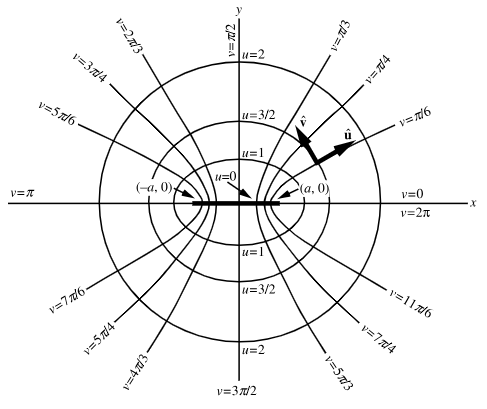
\includegraphics[scale=0.5]{Imagenes/EllipticCylindricalCoord_1000.png}
    \caption{Sistema coordenado cilíndirco elíptico en el plano $x-y$.}
    \label{fig:figura_coordenada_cilindricas_elipticas}
\end{figure}
La familia de superficies coordenadas son las siguientes:
\begin{enumerate}
\item Cilindros elípticos con $u$ constante, $0 \leq u < \infty$
\item Cilindros hiperbólicos conb $v$ constante, $0 \leq v \leq 2 \, \pi$
\item Planos paralelos al plano $x-y$ con $z$ constante, $-\infty < z < \infty$
\end{enumerate}
Como vemos en la siguiente figura (\ref{fig:figura_coordenada_cilindricas_elipticas_3D}):
\begin{figure}[H]
    \centering
    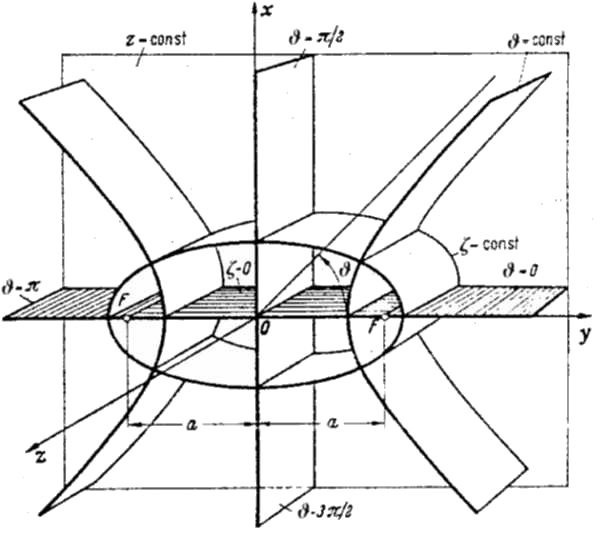
\includegraphics[scale=0.5]{Imagenes/Elliptic-cylindrical-coordinates_02.png}
    \caption{Sistema coordenado cilíndrico elíptico en una vista 3D.}
    \label{fig:figura_coordenada_cilindricas_elipticas_3D}
\end{figure}
\subsection{Factores de escala.}
Calculamos los factores de escala o coeficientes métricos a partir de la expresión:
\begin{align*}
h_{i} &= \abs{\pdv{\vb{r}}{u_{i}}} \\[0.5em]
h_{i} &= \sqrt{ \left( \pdv{x}{u_{i}} \right)^{2} + \left( \pdv{y}{u_{i}} \right)^{2} + \left( \pdv{z}{u_{i}} \right)^{2}}
\end{align*}
Tenemos entonces que
\begin{align*}
h_{1} = h_{u} = \sqrt{ \left( \pdv{x}{u} \right)^{2} + \left( \pdv{y}{u} \right)^{2} + \left( \pdv{z}{u} \right)^{2}}
\end{align*}
donde las derivadas parciales son
\fontsize{12}{12}\selectfont
\begin{align*}
\pdv{x}{u} &= a \, \sinh u \cos v \hspace{0.5cm} \Rightarrow \hspace{0.5cm} \left( \pdv{x}{u} \right)^{2} = a^{2} \, \sinh^{2} u \, \cos^{2} v \\[0.5em]
\pdv{y}{u} &= a \, \cosh u \sin v \hspace{0.5cm} \Rightarrow \hspace{0.5cm} \left( \pdv{y}{u} \right)^{2} = a^{2} \, \cosh^{2} u \, \sin^{2} v \\[0.5em]
\pdv{z}{u} &= 0
\end{align*}
Al sumar los términos del radical
\begin{align*}
h_{u} = \sqrt{a^{2} \, \sinh^{2} u \, \cos^{2} v + a^{2} \, \cosh^{2} u \, \sin^{2} v}
\end{align*}
Haciendo el álgebra respectiva y considerando que $\cosh^{2} u - \sinh^{2} = 1$, entonces tenemos que:
\fontsize{12}{12}\selectfont
\begin{align*}
h_{u} &= \sqrt{a^{2} \left[ \sinh^{2} u \, \cos^{2} v + \cosh^{2} u \, \sin^{2} v \right] } \\[0.5em]
&= \sqrt{a^{2} \left[ \sinh^{2} u \, \cos^{2} v + (1 + \sinh^{2} u) \, \sin^{2} v \right] } \\[0.5em]
&= \sqrt{a^{2} \left[ \sinh^{2} u \, \cos^{2} v + \sinh^{2} u \, \sin^{2} v + \sin^{2} v \right] } \\[0.5em]
&= \sqrt{a^{2} \left[ \sinh^{2} u ( \cos^{2} v + \sin^{2} v ) + \sin^{2} v \right] } \\[0.5em]
&= \sqrt{a^{2} \left[ \sinh^{2} u + \sin^{2} v  \right] }
\end{align*}
\vspace*{-0.6cm}
\begin{align*}
\hspace{-4.5cm}\addtolength{\fboxsep}{5pt}\boxed{
h_{u} = a \, \sqrt{ \sinh^{2} u + \sin^{2} v}}
\end{align*}
Para el factor $h_{v}$ se tiene que:
\fontsize{12}{12}\selectfont
\begin{align*}
h_{v} = \sqrt{ \left( \pdv{x}{v} \right)^{2} + \left( \pdv{y}{v} \right)^{2} + \left( \pdv{z}{v} \right)^{2}}
\end{align*}
Entonces
\fontsize{12}{12}\selectfont
\begin{align*}
\pdv{x}{v} &= - a \, \cosh u \sin v \hspace{0.5cm} \Rightarrow \hspace{0.5cm} \left( \pdv{x}{v} \right)^{2} = a^{2} \, \cosh^{2} u \, \sin^{2} v \\[0.5em]
\pdv{y}{v} &= a \, \sinh u \cos v \hspace{0.5cm} \Rightarrow \hspace{0.5cm} \left( \pdv{y}{v} \right)^{2} = a^{2} \, \sinh^{2} u \, \cos^{2} v \\[0.5em]
\pdv{z}{v} &= 0
\end{align*}
Así llegamos a:
\fontsize{12}{12}\selectfont
\begin{align*}
h_{v} &= \sqrt{a^{2} \left[ \cosh^{2} u \, \sin^{2} v + \sinh^{2} u \, \cos^{2} v \right] } \\[0.5em]
&= \sqrt{a^{2} \left[ (1 + \sinh^{2} u) \, \sin^{2} v + \sinh^{2} u \, \cos^{2} v \right] } \\[0.5em]
&= \sqrt{a^{2} \left[ \sinh^{2} u (\cos^{2} v +  \sin^{2} v)+ \sin^{2} v \right] } \\[0.5em]
&= \sqrt{a^{2} \left[ \sinh^{2} u + \sin^{2} v  \right] }
\end{align*}
\vspace*{-0.35cm}
\begin{equation*}
\hspace{-4.5cm}\addtolength{\fboxsep}{5pt}\boxed{
h_{v} = a \, \sqrt{ \sinh^{2} u + \sin^{2} v}}
\end{equation*}
Para el último factor de escala $h_{z}$:
\fontsize{12}{12}\selectfont
\begin{align*}
h_{z} = \sqrt{ \cancelto{0}{\left( \pdv{x}{z} \right)^{2}} + \cancelto{0}{\left( \pdv{y}{z} \right)^{2}} + \cancelto{1}{\left( \pdv{z}{z} \right)^{2}}}
\end{align*}
\vspace*{-0.35cm}
\begin{equation*}
\hspace{-4.5cm}\addtolength{\fboxsep}{5pt}\boxed{
h_{z} = 1}
\end{equation*}
Los tres factores de escala para este sistema coordenado cilíndrico elíptico son:
\begin{align*}
h_{u} &= a \, \sqrt{ \sinh^{2} u + \sin^{2} v} \\[1em]
h_{v} &= a \, \sqrt{ \sinh^{2} u + \sin^{2} v} \\[1em]
h_{z} &= 1
\end{align*}
\textbf{Ejercicio a cuenta: } Para el sistema de coordenadas esferoidales prolatas $(u, v, \varphi)$, cuyas reglas de transformación son:
\begin{align*}
x &= a \, \sinh u \, \sin v \, \cos \varphi \\
y &= a \, \sinh u \, \sin v \, \sin \varphi \\
z &= a \, \cosh u \, \cos v
\end{align*}
\begin{enumerate}
\item Describe las superficies coordenadas del sistema.
\item Calcula de manera explícita los factores de escala $(h_{u}, h_{v}, h_{\varphi})$.
\end{enumerate}
\section{Cálculo operadores diferenciales.}
\subsection{Gradiente.}
Ya definimos una expresión que nos permitirá calcular el gradiente sobre una función de prueba $\phi$, una vez conocidos los factores de escala del sistema coordenado de interés:
\begin{align*}
\nabla{\phi} = \sum_{i=1}^{3} \dfrac{\vu{e_{i}}}{h_{i}} \, \pdv{\phi}{u_{i}} = \sum_{i=1}^{3} \vu{e}_{i} \left( \nabla{\phi} \right)_{i}
\end{align*}
Por lo que: 
\begin{align*}
\grad{\phi} &= \sum_{i=1}^{3} \dfrac{\vu{e_{i}}}{h_{i}} \, \pdv{\phi}{u_{i}}
\end{align*}
Entonces:
\begin{align*}
\grad{\phi} = \dfrac{1}{a \sqrt{\sinh^{2} u + \sin^{2} v}} \left[ \vu{e}_{u} \pdv{\phi}{u} + \vu{e}_{v} \pdv{\phi}{v} \right] + \vu{e_{z}} \pdv{\phi}{z}
\end{align*}
\subsection{Divergencia.}
Para un campo vectorial $\vb{B}$, habíamos llegado al resultado:
\begin{align*}
\div{\vb{B}} = \dfrac{1}{h} \, \sum_{i=1}^{3} \pdv{u_{i}} \left( \dfrac{B_{i} \, h}{h_{i}} \right)
\end{align*}
donde $h = h_{1} h_{2} h_{3}$


así entonces:
\begin{align*}
\div{\vb{B}} &= \dfrac{1}{h} \left[ \pdv{u} \left( B_{u} \, h_{2} \, h_{3} \right) + \pdv{v} \left( B_{v} \, h_{1} \, h_{3} \right) + \pdv{z} \left( B_{z} \, h_{1} \, h_{2} \right) \right]
\end{align*}
Al realizar las respectivas operaciones y reduciendo las expresiones (tarea moral que puedes hacer), si hacemos $h^{\prime} = \sqrt{\sinh^{2} u + \sin^{2} v}$, tenemos que :
\begin{align*}
\div{\vb{E}} &= \dfrac{1}{a \, h^{\prime}} \left[ \pdv{u} \left( h^{\prime} \, B_{u} \right) + \pdv{v} \left( h^{\prime} \, B_{v} \right) \right] + \pdv{B_{z}}{z}
\end{align*}
\subsection{Rotacional.}
Para calcular el rotacional de un campo vectorial, ocupamos la expresión:
\begin{align*}
\curl{\vb{B}} = \dfrac{1}{h_{1} h_{2} h_{3}} \, \mdet{
h_{1} \, \vu{e}_{1} & h_{2} \, \vu{e}_{2} & h_{3} \, \vu{e}_{3} \\
\displaystyle \pdv{u_{1}} & \displaystyle \pdv{u_{2}} & \displaystyle \pdv{u_{3}} \\
B_{1} \, h_{1} & B_{2} \, h_{2} & B_{3} \, h_{3}
}
\end{align*}
Entonces tendremos que:
Haciendo $h = \sqrt{\sinh^{2} u + \sin^{2} v}$, llegamos a
\begin{align*}
\curl{\vb{B}} &= \dfrac{1}{h^{2}}  \, \mdet{
h \, \vu{e}_{u} & h \, \vu{e}_{v} & \vu{e}_{z} / a \\
\displaystyle \pdv{u_{u}} & \displaystyle \pdv{u_{v}} & \displaystyle \pdv{u_{z}} \\
B_{u} \, h & B_{v} \, h & B_{z} / a
}
\end{align*}
\subsection{Laplaciano}
Para una función escalar $\phi$, definimos el Laplaciano como:
\begin{align*}
\laplacian{\phi} = \dfrac{1}{h} \, \sum_{i=1}^{3} \pdv{u_{i}} \left( \dfrac{h}{h_{i}^{2}}  \pdv{\phi}{u_{i}} \right)
\end{align*}
con $h = h_{1} h_{2} h_{3}$.
Así pues, tenemos que:
\begin{align*}
\laplacian{\phi} = \dfrac{1}{a^{2} \left( \sinh^{2} u + \sin^{2} v \right)} \left[ \pdv[2]{\phi}{u} + \pdv[2]{\phi}{v} \right] + \pdv[2]{\phi}{z}
\end{align*}
\section{Siguiente paso}
\subsection{Construcción de otros sistemas}
Una vez que se ha revisado la metodología para construir sistemas curvilíneos, el siguiente paso sería elaborar la descripción de las superficies coordenadas, calcular los factores de escala, obtener los elementos de línea, superficie y volumen, así como los operadores diferenciales.
\par
De esa manera ya podremos expresar la(s) ecuación(es) que definen un problema de la física bajo una geometría en particular. Esa tarea se desarrollará cuando se nos presente un problema específico.
\par
\textbf{Ejercicio a cuenta: } Ocupando el mismo el sistema de coordenadas esferoidales prolatas $(u, v, \varphi)$ del ejercicio a cuenta anterior:
\begin{enumerate}
\item Calcula los operadores diferenciales $\grad{\phi}$, $\div{\vb{B}}$, $\curl{\vb{B}}$ y $\laplacian{\phi}$
\end{enumerate}
\end{document}